\chapter{CURRENT ECONOMICS}
\begin{chapquote}{Giuliano Amato}
``The treaty clause that triggers exit from the European Union was not actually designed to be used.''
\end{chapquote}

As the quote above suggests, this chapter was not designed to be used because the topics presented in the videos are already explained in the previous chapters. They are the "Housing price conundrum", the "Credit crisis" with MBSs, CDOs and so on, the "Paulson bailout". There are new topics, though, about the European Union and the unemployment, but they won't be reported here for now.

I'll use this chapter to keep track and to explain---to me and to the reader---what is happening right now (from April 2018) in finance and economics.

\section{Yield curve: flattening or inversion?}
Sources: \citep{yield_inversion}

\hspace*{-1cm}
\begin{figure}
\makebox[\textwidth][c]{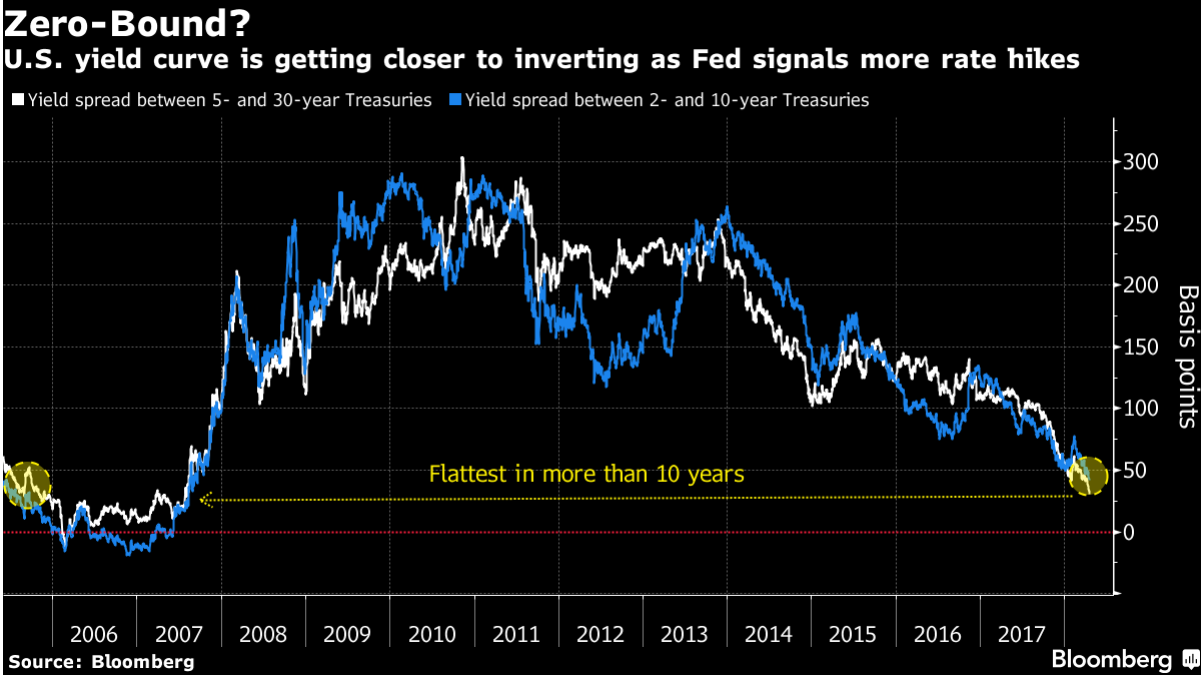
\includegraphics[width=1.3\textwidth]{images/flattening_yields.png}}
    \caption{Different yield spreads in April 2018, when the risk of yield curve inversion is real. We are reaching levels similar to the 2007 financial crisis. Not a good sign.}
    \label{fig:flattening_yields}
\end{figure}
\hspace*{-1cm}

“A potential curve inversion should be taken as seriously as always,” Citigroup analysts led by Jabaz Mathai wrote in an April 13 report. “The historical relationship between the curve and implied recession probabilities is highly non-linear: implied probabilities grow very fast when the curve moves into inverted territory.” Mathai argued that the Fed is wrong on the yield curve, again. He noted that in 2006, then-Chairman Ben S. Bernanke said he didn’t see inversion as portending an economic slowdown.

In the report, Mathai argued that the Fed is wrong on the yield curve, again. He noted that in 2006, then-Chairman Ben S. Bernanke said he didn't see inversion as portending an economic slowdown.

Last month, current Chairman Jerome Powell said “there are good questions about what a flat yield curve or inverted yield curve does to intermediation.” Though he added: “I don’t think that recession probabilities are particularly high right now.”